\documentclass[12pt,letterpaper,titlepage]{article}

%% Language and font encodings
\usepackage[english]{babel}
\usepackage[utf8x]{inputenc}
\usepackage[T1]{fontenc}
\usepackage{caption}
%% Sets page size and margins
%%\usepackage[a4paper,top=3cm,bottom=2cm,left=3cm,right=3cm,marginparwidth=1.75cm]{geometry}

%% Useful packages
\usepackage{amsmath}
\usepackage{graphicx}
\usepackage[colorinlistoftodos]{todonotes}
\usepackage[colorlinks=true, allcolors=blue]{hyperref}
\usepackage{physics}

\title{Project 2: Numerical Modeling of 1-D 2-Phase Radial Flow}
\author{Abdullah A. Alghamdi}


\begin{document}
\maketitle

\renewcommand{\abstractname}{Executive Summary}
\begin{abstract}
Numerical simulation is a key method that the industry adapted to predict reservoir performance over time. This report will investigate one method to model 1-D radial flow in a dual phase reservoir. The simulation model will consist of 1 well and a cylindrical reservoir and a large qualifier around the reservoir. Pressure distribution in the reservoir was calculated implicitly. Furthermore, Saturation distribution was found using explicit discretization. Last but not least, rate forecast was determined using the calculated pressure and saturation. The rates were validated using material balance. The objective of the paper is to build a numerical simulator for a 2-phase reservoir system.
\end{abstract}
\tableofcontents
\pagebreak
\listoffigures
\pagebreak
\section{Model Preparation}
\subsection{Model Description}
An oil reservoir is approximated by 1-D cylindrical formation of one layer, with a constant thickness of $h=50 \,\text{ft}$, as shown in Figure~\ref{fig:1}. The reservoir has radius of $r_e=1500 \,\text{ft}$ where the well bore radius is assumed to be $r_w=100 \,\text{ft}$ for stability purposes. The formation is homogeneous with porosity of $\phi(P_i)=0.2$, permeability of $k=100 \,\text{mD}$, and compressibility of $c_\phi=1\times10^{-5} \,\text{psi}^{-1}$. Before any oil was flown out of the well, the initial reservoir pressure was $P\mid_{t=0}=3000 \,\text{psi}$.
As for fluid properties, the under-saturated oil has a viscosity of $\mu_o=2 \,\text{cp}$, initial formation volume factor of $B_o(P_i)=1.25 \,\text{RB/STB}$, and is slightly compressible with constant coefficient of $c_o=1.5\times10^{-5} \,\text{psi}^{-1}$. Since the reservoir is a 2-phase system, water has a viscosity of $\mu_w=1 \,\text{cp}$, initial formation volume factor of $B_w(P_i)=1.05 \,\text{RB/STB}$, and is slightly compressible with constant coefficient of $c_w=3\times10^{-6} \,\text{psi}^{-1}$. Initial water saturation in the reservoir is $S_w(P_i)=0.25$ and by definition $S_o(P_i)=1-S_w(P_i)=0.75$. The water saturation in the aquifer is always $S_w(P_i)\mid_{r=r_n}=1$.
For simplification purposes, capillary pressure effects were not considered in this model.

\begin{figure}[h]
\centering
\includegraphics[width=.8\textwidth]{Capture.png}
\caption{\label{fig:1}Reservoir model description}
\end{figure}

\subsection{Fluid Originally in Place}
As a benchmark for the rate prediction that the model will generate, it is advisable to calculate the oil and water original in place ($OIIP$ and $WIIP$ respectively). $OIIP$ was found to be $7,522,700$ STB and $WIIP$ was found to be $2,985,200$ STB.
\begin{equation}
OIIP = \frac{\pi h \phi_i S_{oi}(r_e^2-r_w^2)}{5.615\times B_{oi}}
\end{equation}
\begin{equation}
WIIP = \frac{\pi h \phi_i S_{wi}(r_e^2-r_w^2)}{5.615\times B_{wi}}
\end{equation}

\subsection{Relative Permeability}
Since the system has two phases fluids, the relative permeability of each phase should be considered. In the initial condition, $S_w(P_i)=0.25$ which as can be seen from the equations below gives $K_{rw}=0$ which indicate immobile water. However, as water saturation increases, the water relative permeability increases and oil's relative permeability decreases as it can be seen from Figure \ref{Kr}.

\begin{equation}
K_{ro}=
\left\{
		\begin{array} {ll}
        	1.77(1-S_w)^2 & 0.25<S_w \leq 1 \\
            1			& S_w \leq 0.25
         \end{array}
\right.         
\end{equation}
\begin{equation}
K_{rw}=
\left\{
		\begin{array} {ll}
        	2.37(S_w-0.25)^3 & 0.25<S_w \leq 1 \\
            0			& S_w \leq 0.25
         \end{array}
\right.         
\end{equation}

\subsection{Pressure Dependent Variables}
Several variables in this model changes with pressure. Both of water and oil formation volume factors ($B_o$ and $B_w$) increases as pressure decreases. On the other hand, porosity decreases as the pressure decreases. The relationships can be seen in the figures below.
\begin{align}
B_o(P)&=B_{oi}\,e^{-c_o(P-P_i)}\\
B_w(P)&=B_{wi}\,e^{-c_w(P-P_i)}\\
\phi(P)&=\phi_{i}\,e^{-c_\phi(P-P_i)}
\end{align}

\subsection{Mobility Calculations}
oil and water mobilities $\lambda_o$ and $\lambda_w$ are calculated for each cell (i). The mobility has to be averaged between two cells in the right and the left. Thus forming average mobility that is annotated by $\lambda_oW$ and $\lambda_oE$. It can be calculated using the equations below. It is important to use upstream water saturation when calculating $K_{ro}$ and $K_{rw}$. Upstream cell is cell that fluid flow from.
\begin{equation}
\label{moboW}
\lambda_{oW}=\frac{k_avg*K_{ro}Sw_{up}}{\mu_o*Bo_avg}
\end{equation}
\begin{equation}
\label{mobwW}
\lambda_{wW}=\frac{k_avg*K_{rw}Sw_{up}}{\mu_w*Bw_avg}
\end{equation}
\begin{equation}
\label{moboE}
\lambda_{oE}=\frac{k_avg*K_{ro}Sw_{up}}{\mu_o*Bo_avg}
\end{equation}
\begin{equation}
\label{mobwE}
\lambda_{wW}=\frac{k_avg*K_{rw}Sw_{up}}{\mu_w*Bw_avg}
\end{equation}
\subsection{Radial Flow Equation and Boundary Conditions }
radial flow can be modeled using diffusivity equation (see equations \ref{eq:1} and \ref{eq:divw})
which is derived by using mass conservation and Darcy's law. The derivation of this equation includes number of assumptions that have to be mentioned. It is assumed that:
\begin{itemize}
\item mass conservation is applicable,
\item Darcy law is applicable,
\item fluids are slightly compressible,
\item pressure gradient ($\dv{P}{r}$) is small
\item compressibility $C_o$ and $C_\phi$ are constants,
\item permeability is isotropic,
\item viscosity $\mu$ is independent of pressure and radius,
\item thickness $h$ is constant,
\item no vertical flow ($k_z=0$),
\item gravity and capillary pressure effects are ignored.
\end{itemize}

\begin{equation}\label{eq:1}
\pdv{}{r}\left[\lambda_o(r\pdv{P}{r})\right] = 158 r\, \pdv{}{t}\left(\phi \frac{S_o}{B_o}\right)
\end{equation}
\begin{equation}\label{eq:divw}
\pdv{}{r}\left[\lambda_w(r\pdv{P}{r})\right] = 158 r\, \pdv{}{t}\left(\phi \frac{S_w}{B_w}\right)
\end{equation}
where $$\lambda_o=\frac{kK_{ro}}{\mu_o B_o}$$ and $$\lambda_w=\frac{kK_{rw}}{\mu_w B_o}$$

Combining equations \ref{eq:1} and \ref{eq:divw} would give us:
\begin{equation}\label{eq:wo}
B_o\pdv{}{r}\left[\lambda_o(r\pdv{P}{r})\right]+ B_w\pdv{}{r}\left[\lambda_w(r\pdv{P}{r})\right] = 158 r\phi c_t\, \pdv{P}{t}
\end{equation}
where $$c_t=c_\phi+c_o S_o+c_w S_w$$
Initial condition:
\begin{equation}
P(r,t)\mid_{t=0}=P_i=3000\,\text{psi}
\end{equation}
Constant Pressure Boundary Conditions:
\begin{align}
P(r,t)\mid_{r=r_A}=&P_e=3000\,\text{psi}\\
P(r,t)\mid_{r=r_w}=&P_{wf}=1000\,\text{psi}
\end{align}

\subsection{Transformation}
The bulk of the pressure changes in radial flow occurs just near the well-bore with pressure changes decreases as the distance from the well-bore increases. Thus to capture these changes, a small $\Delta r$ should be used. However, the smaller the $\Delta r$, the more computing resources are needed. Therefore, several transformation methods can be used to increase the simulation efficiency without losing vital information in the process. In this paper, we will discuss transforming the radial flow equation to the $\chi$ domain where $\chi=\ln{r}$. We will transform the oil diffusivity equation (equation \ref{eq:1}) which should be applied in the same way to the water diffusivity equation (equation \ref{eq:divw}).
\begin{equation*}
\tag{\ref{eq:wo}}
B_o\pdv{}{r}\left[\lambda_o(r\pdv{P}{r})\right]+ B_w\pdv{}{r}\left[\lambda_w(r\pdv{P}{r})\right] = 158 r\phi c_t\, \pdv{P}{t}
\end{equation*}
Let $$\chi=\ln{(r)}\qquad \Rightarrow \qquad r=e^{\chi}\\$$
%%%%% come back and show work
%\begin{gather*}
%\frac{1}{e^{\chi}}\pdv{}{\chi}\left[e^{\chi}\pdv{P}{\chi}\pdv{\chi}{r}\right] \pdv{\chi}{r}= 158\, \alpha \pdv{P}{t} \\
%B_o\pdv{}{\chi}\left[\lambda_o(\pdv{P}{\chi})\right]+ B_w\pdv{}{\chi}\left[\lambda_w(\pdv{P}{\chi})\right] = 158\, e^{2 \chi}\phi c_t\, \pdv{P}{t}\\
%\end{gather*}
\begin{equation}\label{eq:2}
B_o\pdv{}{\chi}\left[\lambda_o(\pdv{P}{\chi})\right]+ B_w\pdv{}{\chi}\left[\lambda_w(\pdv{P}{\chi})\right] = 158\, e^{2 \chi}\phi c_t\, \pdv{P}{t}
\end{equation} 
Transforming initial condition:
\begin{equation}
P(\chi,t)\mid_{t=0}=P_i=3000\,\text{psi}
\end{equation}
Transforming constant pressure boundary conditions:
\begin{gather}
P(\chi,t)\mid_{\chi=\chi_A}=P_e=3000\,\text{psi}\\
P(\chi,t)\mid_{\chi=\chi_w}=P_{wf}=1000\,\text{psi}
\end{gather}

\subsection{Discretization}
In this model, we are using Implicit Pressure, Explicit Saturation (IMPES) method to model both pressure and saturation changes. The steps of this methods are:
\begin{enumerate}
\item At new time step $n+1$, calculate $K_{ro}$;$K_{rw}$ based on old time $S_o^n$ and $S_w$.
\item Calculate matrix coefficients.
\item Solve for pressure $p^{n+1}$ implicitly.
\item Solve for saturation $S_o^{n+1}$ and $S_w^{n+1}$ explicitly.
\item Increase time by 1 time step and go to step 1.
\end{enumerate}
\subsubsection{Implicit Pressure Discretization}
Using block-centered implicit discretization to discretize equation \ref{eq:2}:
\begin{equation*}\tag{\ref{eq:2}}
\left\{B_o\pdv{}{\chi}\left[\lambda_o(\pdv{P}{\chi})\right]\right\}_i^{n+1}+ \left\{B_w\pdv{}{\chi}\left[\lambda_w(\pdv{P}{\chi})\right]\right\}_i^{n+1}   = 158\, \left\{e^{2 \chi_i}\phi c_t\, \pdv{P}{t}\right\}^{n+1}_i
\end{equation*} 
Discretization of left hand side (LHS):
\begin{equation*}
\begin{aligned}
LHS = &B_o^{n}\frac{\lambda_{oW} P_{i-1}^{n+1}-(\lambda_{oW}+\lambda_{oE})P_i^{n+1}+\lambda_{oE} P^{n+1}_{i+1}}{\Delta\chi^2} \\+  &B_w^{n}\frac{\lambda_{wW} P_{i-1}^{n+1}-(\lambda_{wW}+\lambda_{wE})P_i^{n+1}+\lambda_{wE} P^{n+1}_{i+1}}{\Delta\chi^2}
\end{aligned}
\end{equation*}
\begin{equation}
\label{eq:LHS}
\begin{aligned}
LHS = \frac{1}{\Delta\chi^2}& \{(\lambda_{oW}B_o^n+\lambda_{wW}B_w^n)P_{i-1}^{n+1}\\-&\left[B_o^n(\lambda_{oW}+\lambda_{oE})+B_w^n(\lambda_{wW}+\lambda_{wE})\right]P_i^{n+1}\\+&(\lambda_{oE}B_o^n+\lambda_{wE}B_w^n)P_{i+1}^{n+1}\}
\end{aligned}
\end{equation}
Discretization of right hand side (RHS):
\begin{equation}
\label{eq:RHS}
\begin{aligned}
RHS = 158\,e^{2\chi_i}\phi c_t \frac{P_i^{n+1}-P_i^n}{\Delta t}
\end{aligned}
\end{equation}

combining equations \ref{eq:LHS} and \ref{eq:RHS}
\begin{equation*}
\begin{aligned}
\frac{1}{\Delta\chi^2}& \Bigg\{(\lambda_{oW}B_o^n+\lambda_{wW}B_w^n)P_{i-1}^{n+1}\\-&\left[B_o^n(\lambda_{oW}+\lambda_{oE})+B_w^n(\lambda_{wW}+\lambda_{wE})\right]P_i^{n+1}\\+&(\lambda_{oE}B_o^n+\lambda_{wE}B_w^n)P_{i+1}^{n+1}\Bigg\} = 158\,e^{2\chi_i}\phi c_t \frac{P_i^{n+1}-P_i^n}{\Delta t}
\end{aligned}
\end{equation*}
\begin{equation}
\label{eq:3}
\begin{aligned}
& (\lambda_{oW}B_o^n+\lambda_{wW}B_w^n)P_{i-1}^{n+1}\\-&\left[B_o^n(\lambda_{oW}+\lambda_{oE})+B_w^n(\lambda_{wW}+\lambda_{wE})+158\,e^{2\chi_i}\phi c_t \frac{\Delta\chi^2}{\Delta t}\right]P_i^{n+1}\\+&(\lambda_{oE}B_o^n+\lambda_{wE}B_w^n)P_{i+1}^{n+1} = -158\,e^{2\chi_i}\phi c_t \frac{\Delta\chi^2}{\Delta t}P_i^n
\end{aligned}
\end{equation}
Considering boundary conditions:
when $i=1$
\begin{equation}
\label{bou1}
\begin{aligned}
&-\left[B_o^n(8\lambda_{oW}+4\lambda_{oE})+B_w^n(8\lambda_{wW}+4\lambda_{wE})+158\,e^{2\chi_i}\phi c_t \frac{3\Delta\chi^2}{\Delta t}\right]P_1^{n+1}+ 4(\lambda_{oE}B_o^n+\lambda_{wE}B_w^n)P_{2}^{n+1} \\&= -158\,e^{2\chi_i}\phi c_t \frac{3\Delta\chi^2}{\Delta t}P_i^n-8(\lambda_{oW}B_o^n+\lambda_{wW}B_w^n)P_{wf}^{n+1}
\end{aligned}
\end{equation}
when $i=N$
\begin{equation}
\label{bouN}
\begin{aligned}
&4(\lambda_{oW}B_o^n+\lambda_{wW}B_w^n)P_{N-1}^{n+1}-\left[B_o^n(4\lambda_{oW}+8\lambda_{oE})+B_w^n(4\lambda_{wW}+8\lambda_{wE})+158\,e^{2\chi_i}\phi c_t \frac{3\Delta\chi^2}{\Delta t}\right]P_N^{n+1} \\&= -158\,e^{2\chi_i}\phi c_t \frac{3\Delta\chi^2}{\Delta t}P_N^n- 8(\lambda_{oE}B_o^n+\lambda_{wE}B_w^n)P_{e}^{n+1}
\end{aligned}
\end{equation}
to simplify equations \ref{eq:3}, \ref{bou1}, and and \ref{bouN}:\\
%since $P^n_i=P\mid_{t=0}$
\begin{equation}
\label{abcd}
a P^{n+1}_{i-1}+b P^{n+1}_{i}+c P^{n+1}_{i+1} =d^{n+1}_i
\end{equation}
where: 
\begin{align*}
a\mid_{i=1}&=0\\
a\mid_{i=2:N-1} &=\lambda_{oW}B_o^n+\lambda_{wW}B_w^n\\
a\mid_{i=N} &=4(\lambda_{oW}B_o^n+\lambda_{wW}B_w^n)\\
b\mid_{i=1}&=-\left[B_o^n(8\lambda_{oW}+4\lambda_{oE})+B_w^n(8\lambda_{wW}+4\lambda_{wE})+158\,e^{2\chi_i}\phi c_t \frac{3\Delta\chi^2}{\Delta t}\right]P_1^{n+1}\\
b\mid_{i=2:N-1} &=-\left[B_o^n(\lambda_{oW}+\lambda_{oE})+B_w^n(\lambda_{wW}+\lambda_{wE})+158\,e^{2\chi_i}\phi c_t \frac{\Delta\chi^2}{\Delta t}\right]\\
b\mid_{i=N} &=-\left[B_o^n(4\lambda_{oW}+8\lambda_{oE})+B_w^n(4\lambda_{wW}+8\lambda_{wE})+158\,e^{2\chi_i}\phi c_t \frac{3\Delta\chi^2}{\Delta t}\right]P_N^{n+1}\\
c\mid_{i=1}&=4(\lambda_{oE}B_o^n+\lambda_{wE}B_w^n)\\
c\mid_{i=2:N-1} &=\lambda_{oE}B_o^n+\lambda_{wE}B_w^n\\
d\mid_{i=1}&=-158\,e^{2\chi_i}\phi c_t \frac{3\Delta\chi^2}{\Delta t}P_i^n-8(\lambda_{oW}B_o^n+\lambda_{wW}B_w^n)P_{wf}^{n+1}\\
d\mid_{i=2:N-1} &=-158\,e^{2\chi_i}\phi c_t \frac{\Delta\chi^2}{\Delta t}P_i^n\\
d\mid_{i=N} &=-158\,e^{2\chi_i}\phi c_t \frac{3\Delta\chi^2}{\Delta t}P_N^n- 8(\lambda_{oE}B_o^n+\lambda_{wE}B_w^n)P_{e}^{n+1}\\
\end{align*}

\subsubsection{Explicit Saturation Discretization}
Using block-centered explicit discretization to discretize oil part of equation \ref{eq:1}:

\begin{equation*}
\left\{\pdv{}{\chi}\left[\lambda_o(\pdv{P}{\chi})\right]\right\}_i^{n+1}= \left\{158\, e^{2\chi_i}\, \pdv{}{t}\left(\phi \frac{S_o}{B_o}\right)\right\}^{n+1}_i
\end{equation*} 
\begin{equation*}
\frac{\lambda_{oW} P_{i-1}^{n+1}-(\lambda_{oW}+\lambda_{oE})P_i^{n+1}+\lambda_{oE} P^{n+1}_{i+1}}{\Delta\chi^2}=158\,e^{2\chi_i}  \frac{\left(\phi \frac{S_o}{B_o}\right)_i^{n+1}-\left(\phi \frac{S_o}{B_o}\right)_i^n}{\Delta t}
\end{equation*}
\begin{equation*}
\left(\phi \frac{S_o}{B_o}\right)_i^{n+1}=\left(\phi \frac{S_o}{B_o}\right)_i^n +
\frac{\lambda_{oW} P_{i-1}^{n+1}-(\lambda_{oW}+\lambda_{oE})P_i^{n+1}+\lambda_{oE} P^{n+1}_{i+1}}{158\,e^{2\chi_i}\frac{\Delta\chi^2}{\Delta t}}
\end{equation*}
\\
\begin{equation}
\left({S_o}\right)_i^{n+1}=\frac{B_o^{n+1}}{\phi^{n+1}}\Bigg\{\left(\phi \frac{S_o}{B_o}\right)_i^n +
\frac{\lambda_{oW} P_{i-1}^{n+1}-(\lambda_{oW}+\lambda_{oE})P_i^{n+1}+\lambda_{oE} P^{n+1}_{i+1}}{158\,e^{2\chi_i}\frac{\Delta\chi^2}{\Delta t}}\Bigg\}
\end{equation}
in the same way we find $S_w^{n+1}$
\begin{equation}
\left({S_w}\right)_i^{n+1}=\frac{B_w^{n+1}}{\phi^{n+1}}\Bigg\{\left(\phi \frac{S_w}{B_w}\right)_i^n +
\frac{\lambda_{wW} P_{i-1}^{n+1}-(\lambda_{wW}+\lambda_{wE})P_i^{n+1}+\lambda_{wE} P^{n+1}_{i+1}}{158\,e^{2\chi_i}\frac{\Delta\chi^2}{\Delta t}}\Bigg\}
\end{equation}

Considering boundary conditions, when $i=1$ or $i=N$:
\begin{equation}
\label{so}
\left({S_o}\right)_i^{n+1}=\frac{B_o^{n+1}}{\phi^{n+1}}\Bigg\{\left(\phi \frac{S_o}{B_o}\right)_i^n +
\frac{8\lambda_{oW} P_{i-1}^{n+1}-(8\lambda_{oW}+4\lambda_{oE})P_i^{n+1}+4\lambda_{oE} P^{n+1}_{i+1}}{158\,e^{2\chi_i}\frac{3\Delta\chi^2}{\Delta t}}\Bigg\}
\end{equation}
\begin{equation}
\label{sw}
\left({S_w}\right)_i^{n+1}=\frac{B_w^{n+1}}{\phi^{n+1}}\Bigg\{\left(\phi \frac{S_w}{B_w}\right)_i^n +
\frac{8\lambda_{wW} P_{i-1}^{n+1}-(8\lambda_{wW}+4\lambda_{wE})P_i^{n+1}+4\lambda_{wE} P^{n+1}_{i+1}}{158\,e^{2\chi_i}\frac{3\Delta\chi^2}{\Delta t}}\Bigg\}
\end{equation}

%%%%%%%%%%%%%%%%%%%%%%%%%%%%%%%%%%%%%%%%%%%%%
\section{Scenario 1: 4 cells and 1 time step ($k=10$ md and $rw=0.25$ ft) }

In the first scenario, the flow path will be divided to 4 center blocks cells ($N=4$) with spacing of $\Delta\chi$ as shown in Figure \ref{fig:2}. This simulation instance will be limited to 1 time step of 1 day ($t=1$ and $\Delta t=1$). In scenario 1, permeability $k=10$ md and $rw=0.25$ ft.  


\begin{gather}\label{eq:dx}
\Delta\chi=\frac{\ln{r_e}-\ln{r_w}}{n-1}\\\label{eq:dx2}
\chi_i=\ln{r_w}+\frac{2i-1}{2}\Delta\chi\\\label{eq:dx3}
\chi_{N+1}=\chi_N+\frac{1}{2}\Delta\chi
\end{gather}
\begin{table}[h]
\centering
\begin{tabular}{lrrr}
$i$  & $\chi_i$ [ft]& Radius ($r_i$) [ft]  \\\hline
0 &4.6052 & 100.00\\
1& 5.0565 & 157.00\\
2& 5.9592 & 387.30\\
3 &6.8619 & 955.20\\
4& 7.7646 & 2355.6\\
5& 8.2159 & 3699.4\\
\hline
\end{tabular}
\caption{\label{tab:4}$\chi_i$ and $r_i$ for $i=0-5$}
\end{table}

\begin{figure}[p]
\centering
\includegraphics[width=0.7\textwidth]{Capture2.PNG}
\caption{\label{fig:2}Schematic of simulation cells}
\end{figure}
First, average mobilities $\lambda_o$, $\lambda_w$ have to be calculated based on the initial saturations and pressures using equations \ref{moboW},\ref{mobwW},\ref{moboE}, and \ref{mobwE}.
\begin{gather*}
\lambda_{oW}= [3.9232,4,4,0]		\\
\lambda_{wW}= [0,0,0,9.5223]		\\
\lambda_{oE}= [4,4,0,0]		\\
\lambda_{wE}= [0,0,9.5223,9.5223]		\\
\end{gather*}


Using equation \ref{abcd} we can find a,b,c, and d for i=1,2,3, and 4.

\underline{when $i=1$:}\\
\begin{equation*}
b_1 P^{n+1}_{1}+c_1 P^{n+1}_{2} =d^{n+1}_1
\end{equation*}
where: 
\begin{align*}
a_1&=0\\
b_1&=-\left[B_o^n(8\lambda_{oW}+4\lambda_{oE})+B_w^n(8\lambda_{wW}+4\lambda_{wE})+158\,e^{2\chi_1}\phi c_t \frac{3\Delta\chi^2}{\Delta t}\right]P_1^{n+1}\\
c_1&=4(\lambda_{oE}B_o^n+\lambda_{wE}B_w^n)\\
d_1&=-158\,e^{2\chi_1}\phi c_t \frac{3\Delta\chi^2}{\Delta t}P_1^n-8(\lambda_{oW}B_o^n+\lambda_{wW}B_w^n)P_{wf}^{n+1}\\
\end{align*}

\underline{when $i=2$:}
\begin{equation*}
a_2 P^{n+1}_{1}+b_2 P^{n+1}_{2}+c_2 P^{n+1}_{3} =d^{n+1}_2
\end{equation*}
where: 
\begin{align*}
a_2 &=\lambda_{oW}B_o^n+\lambda_{wW}B_w^n\\
b_2 &=-\left[B_o^n(\lambda_{oW}+\lambda_{oE})+B_w^n(\lambda_{wW}+\lambda_{wE})+158\,e^{2\chi_2}\phi c_t \frac{\Delta\chi^2}{\Delta t}\right]\\
c_2 &=\lambda_{oE}B_o^n+\lambda_{wE}B_w^n\\
d_2 &=-158\,e^{2\chi_2}\phi c_t \frac{\Delta\chi^2}{\Delta t}P_2^n\\
\end{align*}

\underline{when $i=3$:}
\begin{equation*}
a_3 P^{n+1}_{2}+b_3 P^{n+1}_{3}+c_3 P^{n+1}_{4} =d^{n+1}_3
\end{equation*}
where: 
\begin{align*}
a_3 &=\lambda_{oW}B_o^n+\lambda_{wW}B_w^n\\
b_3 &=-\left[B_o^n(\lambda_{oW}+\lambda_{oE})+B_w^n(\lambda_{wW}+\lambda_{wE})+158\,e^{2\chi_3}\phi c_t \frac{\Delta\chi^2}{\Delta t}\right]\\
c_3 &=\lambda_{oE}B_o^n+\lambda_{wE}B_w^n\\
d_3 &=-158\,e^{2\chi_3}\phi c_t \frac{\Delta\chi^2}{\Delta t}P_3^n\\
\end{align*}

\underline{when $i=4$:}\\
\begin{equation*}
a_4 P^{n+1}_{3}+b_4 P^{n+1}_{4}=d^{n+1}_4
\end{equation*}
where:
\begin{align*}
a_4 &=4(\lambda_{oW}B_o^n+\lambda_{wW}B_w^n)\\
b_4 &=-\left[B_o^n(4\lambda_{oW}+8\lambda_{oE})+B_w^n(4\lambda_{wW}+8\lambda_{wE})+158\,e^{2\chi_4}\phi c_t \frac{3\Delta\chi^2}{\Delta t}\right]P_4^{n+1}\\
d_4 &=-158\,e^{2\chi_4}\phi c_t \frac{3\Delta\chi^2}{\Delta t}P_4^n- 8(\lambda_{oE}B_o^n+\lambda_{wE}B_w^n)P_{e}^{n+1}
\end{align*}

The matrix coefficients forms 4X4  tridiagonal matrix that can be solved using Thomas Algorithm:



\renewcommand{\arraystretch}{2}
 \[ \begin{aligned}
    & \begin{bmatrix} 
     b_1 & c_1 & 0 & 0 \\ 
     a_2 & b_2 & c_2 & 0 \\
        0 &  a_3 & b_3 & c_3 \\
       0&0&a_4& b_4
 \end{bmatrix} 
  \times \begin{bmatrix} 
      P^{n+1}_1        \\ 
      P^{n+1}_2        \\ 
      P^{n+1}_3        \\ 
      P^{n+1}_4        \\ 
    \end{bmatrix} &= \left[\begin{array}{l}  d_1\\d_2\\d_3\\d_4  \end{array}\right]
\end{aligned}  \] 



\subsection{Results and Discussion}
Table \ref{tab:1} shows the solution of the discretized equations using Thomas Algorithm. It can be seen the effect of the transformation on the cell sizes where as the distance from the well-bore increases, the larger the size of the cell becomes. This, however, could have the drawback of reduced resolution as the radius increases. Oil and Water saturation were also calculated using the new time calculated pressures.The summation of the saturation were check to be equal to 1 as a validity check. It can be seen from the table that the changes in saturation were minor because the short simulation time. In the next scenario we can examine the change in saturation more clearly. 
\begin{table}[h]
\centering
\begin{tabular}{lrrrrr}
$i$  & $\chi_i$ [ft]& $r_i$ [ft] & $P_i^{n+1}$ [psi] & Oil  $S_{oi}^{n+1}$ & $Sw_i^{n+1}$\\\hline
0 &-1.3863 & 0.25&	1000.0& - & -\\
1& 0.0636 & 1.07&	1460.8&0.7442 &0.2551\\
2& 2.9635 & 19.36&	2367.0&0.7478 &0.2521\\
3 &5.8633 & 351.8&2995.7&0.7500 &0.2500\\
4& 8.7631 & 6351.9&	3000&0 &1\\
5& 10.213 & 27000&	3000.0&0 &1\\
\hline
\end{tabular}
\caption{\label{tab:1}Results of the 4 unknown pressures}
\end{table}
\pagebreak


\section{Scenario 2: 4 cells and 1 time step ($k=100$ md and $rw=100$ ft) }
This is almost identical scenario to the previous one. However, permeability were changed back to 100 md and well radius was increased to 100 ft. The same simulator was used in this step. Table \ref{100} has the results.

\begin{table}[h]
\centering
\begin{tabular}{lrrrrr}
$i$  & $\chi_i$ [ft]& $r_i$ [ft] & $P_i^{n+1}$ [psi] & Oil  $S_{oi}^{n+1}$ & $Sw_i^{n+1}$\\\hline
0 &4.6052 & 100.00&	1000.0& - & -\\
1& 5.0565 & 157.00&	1643.0&0.745 &0.2544\\
2& 5.9592 & 387.30&	2625.5&0.7487 &0.2515\\
3 &6.8619 & 955.20&2971.7&0.7498 &0.2502\\
4& 7.7646 & 2355.6&	2998.3&0 &1\\
5& 8.2159 & 3699.4&	3000.0&0 &1\\
\hline
\end{tabular}
\caption{\label{100}Results of the 4 unknown pressures}
\end{table}
\pagebreak

\section{Scenario 3: 11 cells and 1000 time steps}
In this scenario, the number of cells will be increased ($N=11$). Therefore, $\Delta\chi$ should be recalculated using Equations \ref{eq:dx}, \ref{eq:dx2} and \ref{eq:dx3}. Moreover, the simulation will show pressure change over 1000 days ($t=1000$) with a time step of 1 day ($\Delta t=1$). The discretized equations are used in a similar way to the last scenario. From Equations \ref{abcd}, 11 equations will be constructed to solve 11 unknown pressures. This step will be repeated 1000 times to model pressure change over time. In each time step, the solved pressures from the old time will be used in $P_i^n$. After that, saturations are calculated using equations \ref{so} and \ref{sw}.
\subsection{Pressure Calculation}

First, average mobilities $\lambda_o$, $\lambda_w$ have to be calculated based on the initial saturations and pressures using equations \ref{moboW},\ref{mobwW},\ref{moboE}, and \ref{mobwE}.Then Using equation \ref{abcd} we can find a,b,c, and d for i=1,2,3, and 4.

\underline{when $i=1$:}\\
\begin{equation*}
b_1 P^{n+1}_{1}+c_1 P^{n+1}_{2} =d^{n+1}_1
\end{equation*}
where:
\begin{align*}
a_1&=0\\
b_1&=-\left[B_o^n(8\lambda_{oW}+4\lambda_{oE})+B_w^n(8\lambda_{wW}+4\lambda_{wE})+158\,e^{2\chi_1}\phi c_t \frac{3\Delta\chi^2}{\Delta t}\right]P_1^{n+1}\\
c_1&=4(\lambda_{oE}B_o^n+\lambda_{wE}B_w^n)\\
d_1&=-158\,e^{2\chi_1}\phi c_t \frac{3\Delta\chi^2}{\Delta t}P_1^n-8(\lambda_{oW}B_o^n+\lambda_{wW}B_w^n)P_{wf}^{n+1}\\
\end{align*}

\underline{when $i=[2,10]$:}
\begin{equation*}
a P^{n+1}_{i-1}+b P^{n+1}_{i}+c P^{n+1}_{i+1} =d^{n+1}_i
\end{equation*}
where:
\begin{align*}
a_i &=\lambda_{oW}B_o^n+\lambda_{wW}B_w^n\\
b_i &=-\left[B_o^n(\lambda_{oW}+\lambda_{oE})+B_w^n(\lambda_{wW}+\lambda_{wE})+158\,e^{2\chi_i}\phi c_t \frac{\Delta\chi^2}{\Delta t}\right]\\
c_i &=\lambda_{oE}B_o^n+\lambda_{wE}B_w^n\\
d_i &=-158\,e^{2\chi_i}\phi c_t \frac{\Delta\chi^2}{\Delta t}P_i^n\\
\end{align*}

\underline{when $i=11$:}\\
\begin{equation*}
a P^{n+1}_{10}+b P^{n+1}_{11} =d^{n+1}_{11}
\end{equation*}
where:
\begin{align*}
a_{11} &=4(\lambda_{oW}B_o^n+\lambda_{wW}B_w^n)\\
b_{11} &=-\left[B_o^n(4\lambda_{oW}+8\lambda_{oE})+B_w^n(4\lambda_{wW}+8\lambda_{wE})+158\,e^{2\chi_{11}}\phi c_t \frac{3\Delta\chi^2}{\Delta t}\right]P_{11}^{n+1}\\
d_{11} &=-158\,e^{2\chi_{11}}\phi c_t \frac{3\Delta\chi^2}{\Delta t}P_{11}^n- 8(\lambda_{oE}B_o^n+\lambda_{wE}B_w^n)P_{e}^{n+1}
\end{align*}

The matrix coefficients forms 11X11  tridiagonal matrix that can be solved using Thomas Algorithm:
 
 \[ \begin{aligned}
    & \begin{bmatrix} 
     b_1 & c_1 &  & &&0 \\ 
     a_2 & b_2 & c_2 && & \\
     & a_3 & b_3 & \ddots&&  \\
         &&  \ddots & \ddots && c_{10} \\
       0&&&a_{11}&& b_{11}
 \end{bmatrix} 
  \times \begin{bmatrix} 
   P^{n+1}_1        \\ 
      P^{n+1}_2        \\ 
      P^{n+1}_{3}        \\ 
      \vdots        \\ 
      P^{n+1}_{11}        \\ 
    \end{bmatrix} &= \left[\begin{array}{l}  d_1\\d_2\\d_3\\\vdots\\d_{11}  \end{array}\right]
\end{aligned}  \]

\subsection{Calculating Saturation}
Now that Pressures $P^{n+1}_{i}$ were calculated, pressure dependent variables has to be updated. Equations 5, 6, 7 were used as shown below.
\begin{align*}
B_{oi}^{n+1}&=B_{oi}^{n}\,e^{-c_o(P_i^{n+1}-P_i^n)}\\
B_{wi}^{n+1}&=B_{wi}^{n}\,e^{-c_w(P_i^{n+1}-P_i^n)}\\
\phi_i^{n+1}&=\phi_{i}^{n}\,e^{-c_\phi(P_i^{n+1}-P_i^n)}
\end{align*}

Then we use the new pressure-dependent variables in equations \ref{so} and \ref{sw} to solve for $S_i^{n+1}$.


\subsection{Results and Discussion}
The 11 unknowns pressures were obtained by using Thomas Algorithm to solve for the discretized equations. Then the process was repeated 1000 times to show pressure changes over time. In each time step, the pressure calculated from the previous time step were used as old time pressure $P_i^n$. The results were plotted in Figure \ref{press}. It can be seen form the figure that pressure decreases as production time increases. However, boundary conditions keep the pressure constant at the well and at the outer boundary. In figure \ref{p12510} pressure changes in the first 30 days are shown clearly.


\section{Rate Forecast}
A rate forecast of scenario 3 is necessary to complete the simulation study. Forecasting rates were approached using equations \ref{qo} and \ref{qw}. These equations use the pressure gradient from the center of the first block ($P_1^{n+1}$)to the pressure on the well-bore sand face ($P_{wf}$) to calculate the rate. 
\begin{equation}
\label{qo}
q_o=7.08\times 10^{-3} \frac{kK_{ro}h}{\mu_o B_o} \frac{P_1^{n+1}-P_{wf}}{0.5 \Delta\chi}
\end{equation}
\begin{equation}
\label{qw}
q_w=7.08\times 10^{-3} \frac{kK_{rw}h}{\mu_w B_w} \frac{P_1^{n+1}-P_{wf}}{0.5 \Delta\chi}
\end{equation}

After calculating the flow rates, water oil ration and water cut can be easily calculated using equations \ref{wor} and \ref{wc}.
\begin{equation}
\label{wor}
WOR=\frac{q_w}{q_o}
\end{equation}
\begin{equation}
\label{wc}
f_w=\frac{q_w}{q_w+q_o}
\end{equation}
Since water is flowing from the aquifer to the well-bore, it is important to find when the water production will start. This time is called water breakthrough time ($tb$) and can be defined as:$$t_b=t\mid_{q_w>0}$$


The next step is calculating cumulative oil production $N_p$ and recovery factor after 1000 days using equations \ref{Np} and \ref{RF}
\begin{equation}
\label{Np}
N_p=\sum_{i=0}^{1000} q_{o}\mid_{t=i}
\end{equation}
\begin{equation}
\label{RF}
RF = \frac{N_p}{OIIP}
\end{equation}

Last but not least, a material balance has to be completed to validate the simulation. Material balance shows the ration between the cumulative production $N_p$ added to the oil in place $OIP$ at a specific time to the original oil in place $OIIP$
$$MBratio=\frac{OIP+N_p}{OIIP}$$

\subsection{Results and Discussion}
The flow rates calculated  plotted in Figures \ref{qo} and \ref{qw}. From Figure \ref{qo}, oil rate decreased rapidly in early production time. Then it continued to decreased until it reached around the 550 days mark when it returned to the rapid decrease rate. From figure \ref{qw}, we can see that the water production started at 574 days mark ($t_b=574$ days) which explains the rapid decreases in the oil production at the same time. Water production skyrocketed reaching more than 8000 STB/day by the end of the simulation. Water Oil Ration (WOR) and Water Cut ($f_w$) reached around 7.2 and 0.88 respectively as can be seen from Figures \ref{wor} and \ref{fw}. 

Recovery fraction after the 1000 days was found to be 0.7475 and 0.6516 at $t_b$. Moreover, Cumulative oil production was calculated ($N_p=5.6235$ MMSTB) after 1000 days and ($N_p=4.9018$ MMSTB).Material balance check was valid with a small deviation of .7 percent expected from the approximation of the numerical simulation (see Figure \ref{mb}). Saturation changes over distance is shown in Figures \ref{so} and \ref{sw}.







\section{Conclusions}

\par this report, the goal was to build a numerical simulator of a 1-D radial flow for 2-phase fluid system. Pressure distribution over distance and time was found.Also, saturation changes were found. Last but not least, rate forecast study was conducted to asses reservoir performance. Material balance were valid.
\begin{figure}[p]
\centering
\makebox[\textwidth][c]{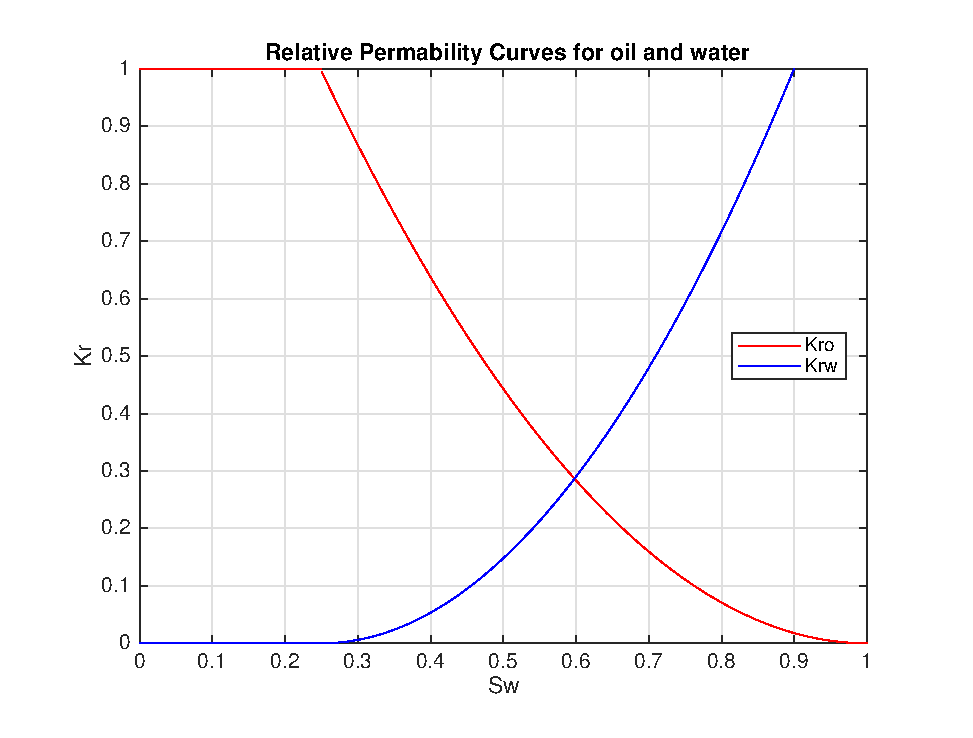
\includegraphics[width=1.5\textwidth]{Kr.eps}}
\caption{\label{Kr}Reltive Permeability Curves}
\end{figure}
\begin{figure}[p]
\centering
\makebox[\textwidth][c]{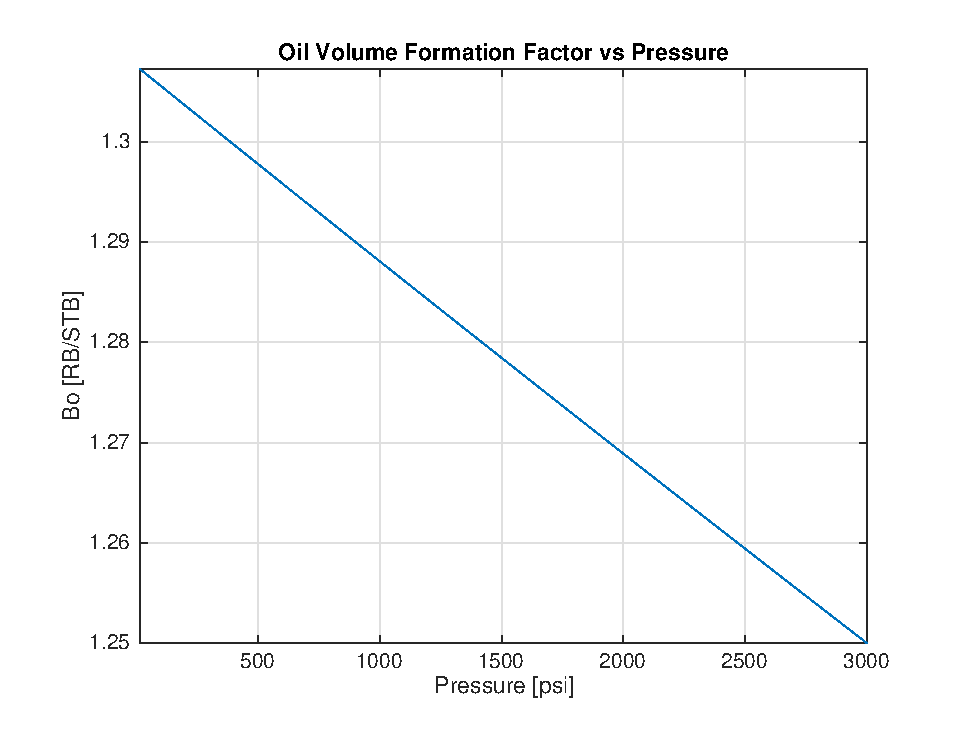
\includegraphics[width=1.5\textwidth]{Bo.eps}}
\caption{\label{Bo}Oil Volume Formation Factor-Pressure Relationship }
\end{figure}
\begin{figure}[p]
\centering
\makebox[\textwidth][c]{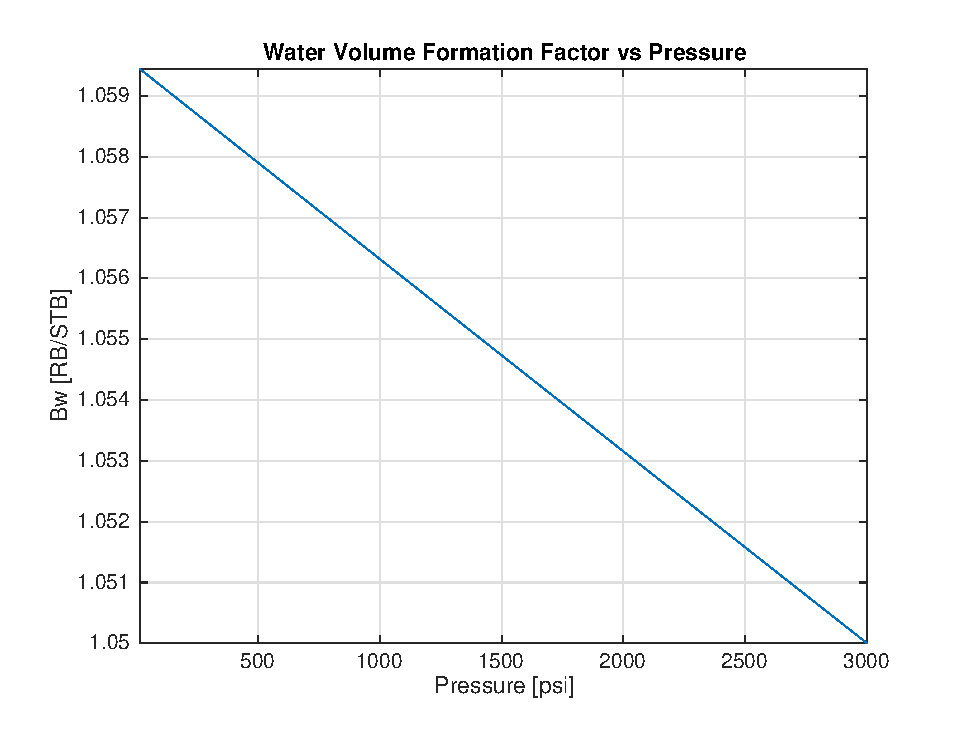
\includegraphics[width=1.5\textwidth]{Bw.eps}}
\caption{\label{Bw}Oil Volume Formation Factor-Pressure Relationship}
\end{figure}
\begin{figure}[p]
\centering
\makebox[\textwidth][c]{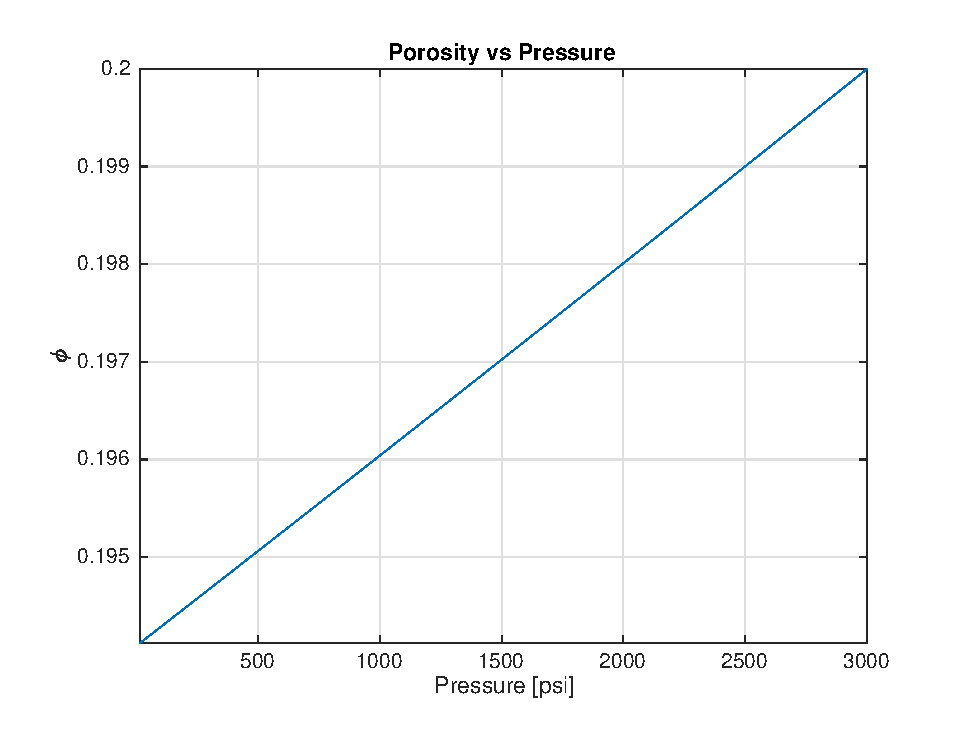
\includegraphics[width=1.5\textwidth]{phi.eps}}
\caption{\label{phi}Porosity-Pressure Relationship}
\end{figure}
\begin{figure}[p]
\centering
\makebox[\textwidth][c]{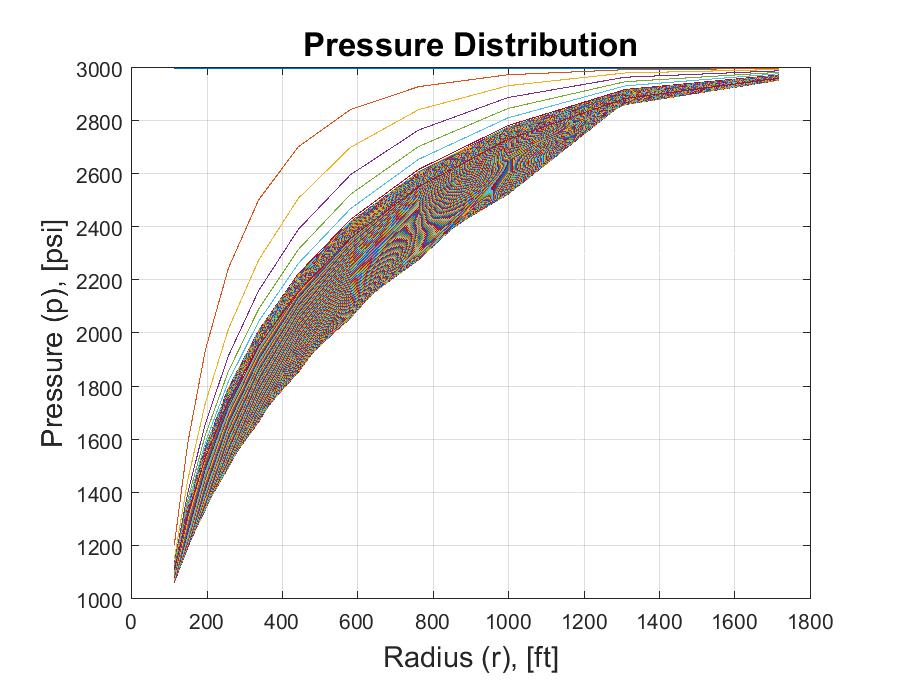
\includegraphics[width=1.5\textwidth]{press.eps}}
\caption{\label{press}Pressure Distribution for scenario 3}
\end{figure}
\begin{figure}[p]
\centering
\makebox[\textwidth][c]{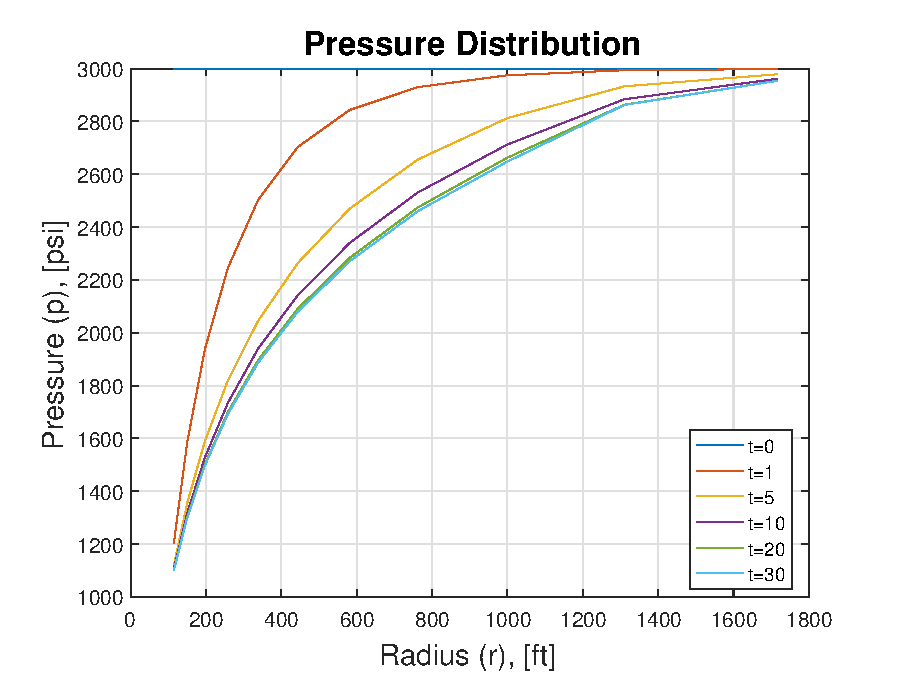
\includegraphics[width=1.5\textwidth]{pre12510.eps}}
\caption{\label{p12510}Pressure Distribution for scenario 3 for 6 selected times}
\end{figure}
\begin{figure}[p]
\centering
\makebox[\textwidth][c]{\includegraphics[width=1.5\textwidth]{qo.eps}}
\caption{\label{qo}Oil Production Rate vs. Time}
\end{figure}
\begin{figure}[p]
\centering
\makebox[\textwidth][c]{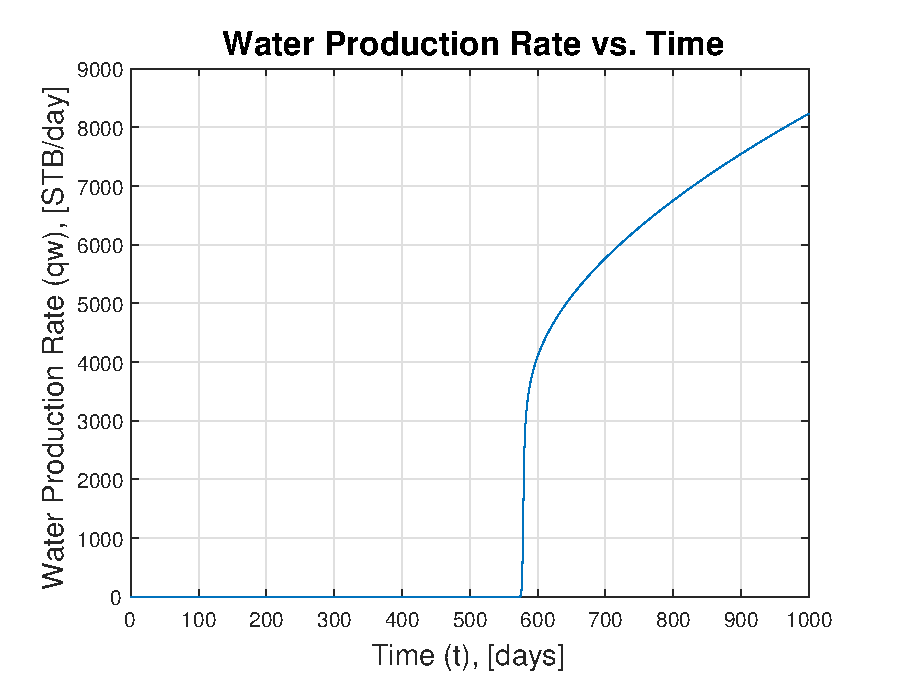
\includegraphics[width=1.5\textwidth]{qw.eps}}
\caption{\label{qw}Water Production Rate vs. Time}
\end{figure}
\begin{figure}[p]
\makebox[\textwidth][c]{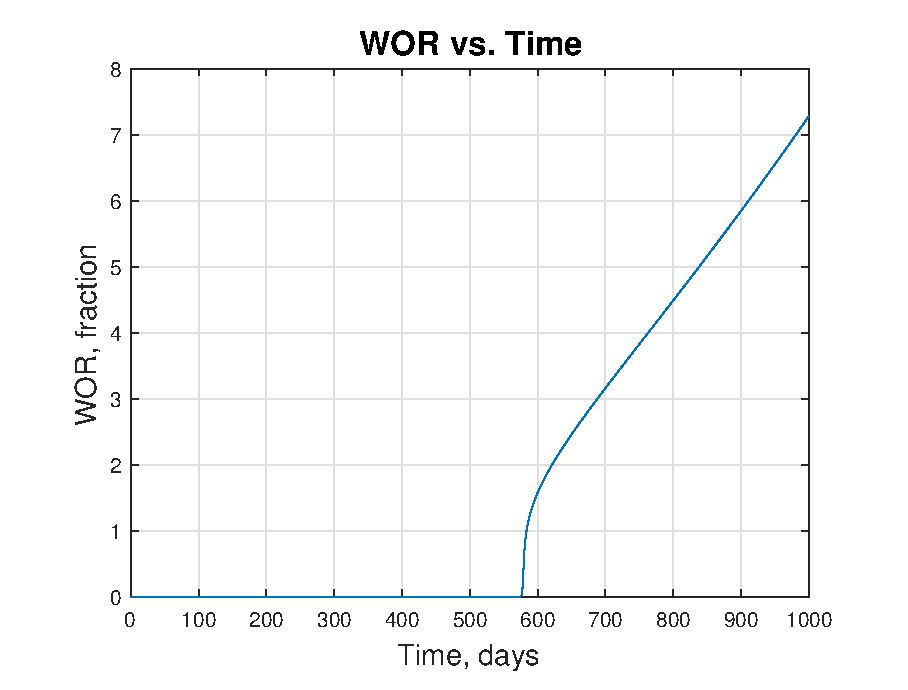
\includegraphics[width=1.5\textwidth]{wor.eps}}
\caption{\label{wor}Water Oil Ratio vs Time}
\end{figure}

\begin{figure}[p]
\makebox[\textwidth][c]{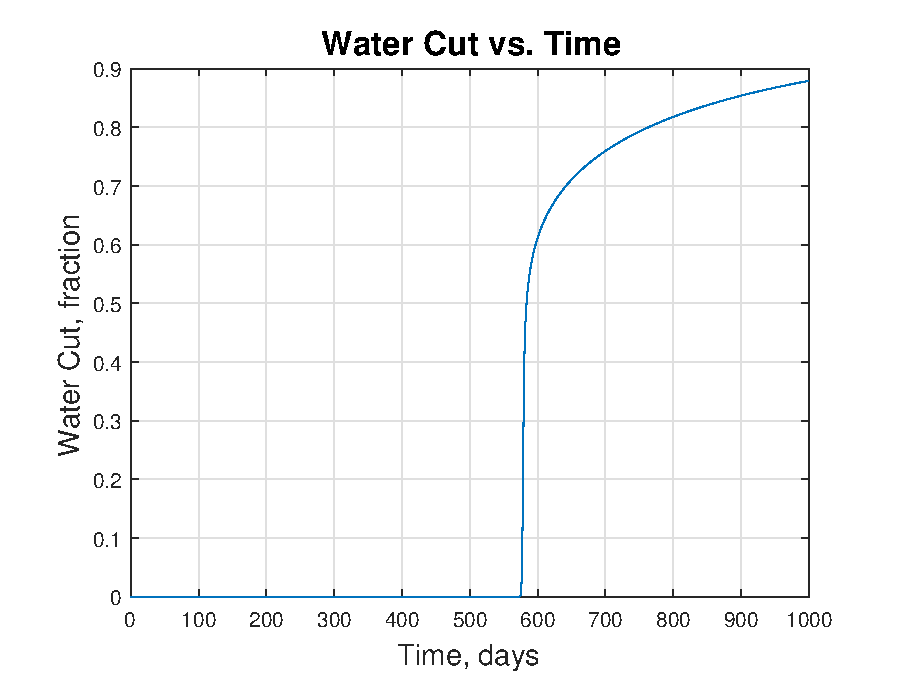
\includegraphics[width=1.5\textwidth]{fw.eps}}
\caption{\label{fw}Water Cut vs Time}
\end{figure}
\begin{figure}[p]
\makebox[\textwidth][c]{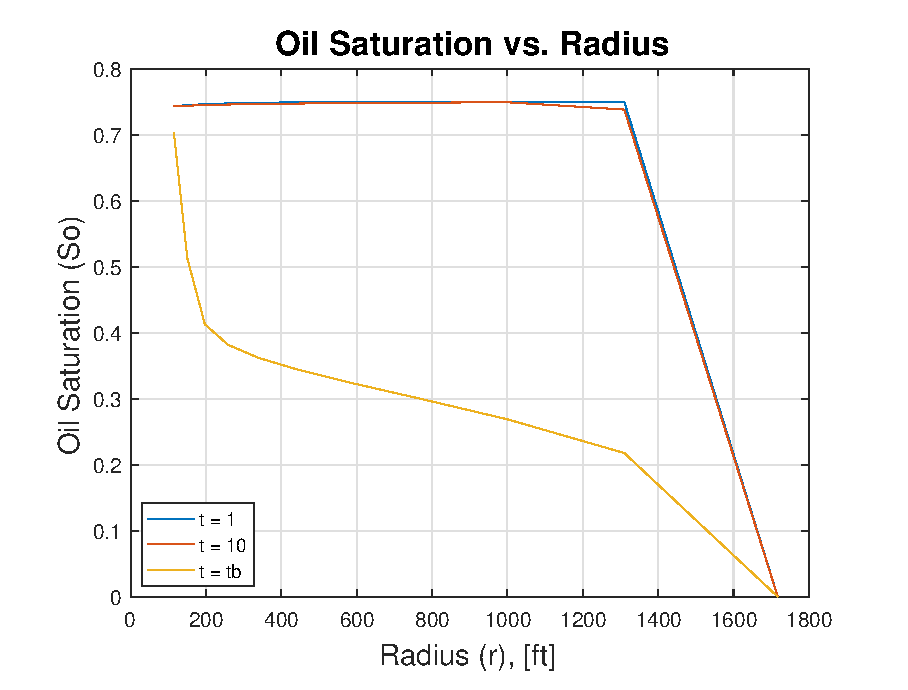
\includegraphics[width=1.5\textwidth]{So.eps}}
\caption{\label{so}Oil Saturation vs Radius}
\end{figure}
\begin{figure}[p]
\makebox[\textwidth][c]{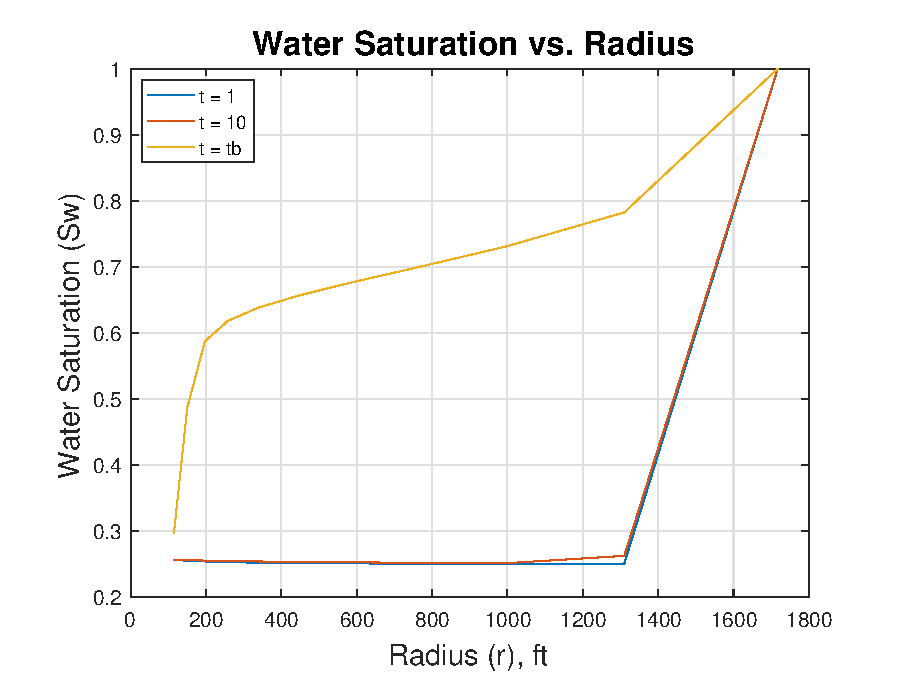
\includegraphics[width=1.5\textwidth]{Sw.eps}}
\caption{\label{sw}Water Saturation vs Radius}
\end{figure}
\begin{figure}[p]
\makebox[\textwidth][c]{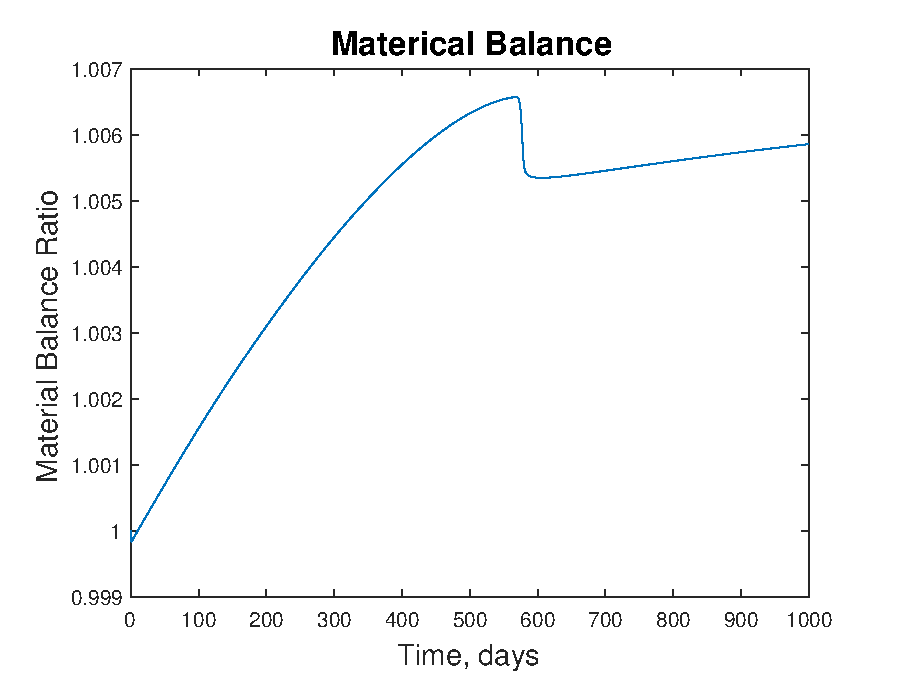
\includegraphics[width=1.5\textwidth]{mb.eps}}
\caption{\label{mb}Material Balance verification (1 is perfect)}
\end{figure}

\pagebreak
\appendix
Matlab R2017a code:
\begin{verbatim}
clear
%to solve for Part 1-5, make n=4 and t=1
t=1000;
n=11;
%initial variables
dt=1;
ts=t/dt; %timestep
re=1500;
rw=100;
h=50;
pi=3000;
pwf=1000;
pe=3000;
k=100;
k_avg=2*k*k/(k+k);
phi_i=0.2;
phi=ones(ts+1,n)*phi_i;
vis_o=2;
vis_w=1;
B_oi=1.25;
B_wi=1.05;
B_o=ones(1,n)*B_oi;
B_w=ones(1,n)*B_wi;
c_f=1e-5;
c_o=1.5e-5;
c_w=0.3e-5;
S_oi=.75;
S_wi=1-S_oi;
% S_w=ones(1,n)*0.25;
% S_w(:,n)=1;
% S_o=1-S_w;
No=0;
Wp=0;
%%%%1. Calculate OIIP %%%%%%
OIIP=(22/7*(re^2-rw^2))*h*phi(1,1)*S_oi/(5.615*B_oi)
%%%%2. Calculate  water initially in place, W %%%%
WIP=(22/7*(re^2-rw^2))*h*phi(1,1)*S_wi/(5.615*B_wi)

%create p array
p=ones(1,n)*pi;

%create X & r arraies
dx=(log(re)-log(rw))/(n-1);
x(1)=log(rw)+.5*dx;
for i=2:n
    x(i) = x(i-1)+dx;
end
r=exp(x);
%inital time
m=1;
for i=1:n
    S_o(m,i)=.75;
    S_w(m,i)=1-S_o(i);
    ct(m,i)=c_f+c_o*S_o(m,i)+c_w*S_w(m,i);
    alpha(m,i)=158*phi(m,i)*ct(m,i);
end
for i=1:1:n
    B_o(m,i)=B_oi*exp(-c_o*(p(m,i)-pi));
    B_w(m,i)=B_wi*exp(-c_w*(p(m,i)-pi));
    phi(m,i)= phi_i*exp(c_f*(p(m,i)-pi));
end
S_o(m,n)=0;
S_w(m,n)=1-S_o(m,n);
ct(m,n)=c_f+c_o*S_o(m,n)+c_w*S_w(m,n);
alpha(m,n)=158*phi(m,n)*ct(m,n);
%%%%%% Computing lamdas

% Computing West lamdas

for i=n:-1:2
    if(p(m,i-1)>p(m,i))
        SwUp(m,i)=S_w(m,i-1);
    else
        SwUp(m,i)=S_w(m,i);
    end
    
    B_oAvg(m,i)=B_oi*exp(-c_o*(((p(m,i-1)+p(m,i))/2)-pi));
    B_wAvg(m,i)=B_wi*exp(-c_w*(((p(m,i-1)+p(m,i))/2)-pi));
    if(SwUp(m,i)<=.25)
        kro(m,i)=1;
        krw(m,i)=0;
        l_o_W(m,i)=k*kro(m,i)/(vis_o*B_oAvg(m,i));
        l_w_W(m,i)=k*krw(m,i)/(vis_w*B_wAvg(m,i));
    else
        kro(m,i)=(1.77*(1-SwUp(m,i))^2);
        krw(m,i)=(2.37*(SwUp(m,i)-.25)^3);
        l_o_W(m,i)=k*kro(m,i)/(vis_o*B_oAvg(m,i));
        l_w_W(m,i)=k*krw(m,i)/(vis_w*B_wAvg(m,i));
    end
end
SwUp(m,1)=S_w(m,1);
B_oAvg(m,1)=B_oi*exp...
    (-c_o*(((pwf+p(m,1))/2)-pi));
B_wAvg(m,1)=B_wi*exp...
    (-c_w*(((pwf+p(m,1))/2)-pi));
if(SwUp(m,1)<=.25)
    kro(m,1)=1;
    krw(m,1)=0;
else
    kro(m,1)=(1.77*(1-SwUp(m,1))^2);
    krw(m,1)=(2.37*(SwUp(m,1)-.25)^3);
end
l_o_W(m,1)=k*kro(m,1)/(vis_o*B_oAvg(m,1));
l_w_W(m,1)=k*krw(m,1)/(vis_w*B_wAvg(m,1));


% Computing East lamdas

for i=n-1:-1:1
    if(p(m,i)>p(m,i+1))
        SwUp(m,i)=S_w(m,i+1);
    else
        SwUp(m,i)=S_w(m,i);
    end
    
    B_oAvg(m,i)=B_oi*exp(-c_o*(((p(m,i+1)+p(m,i))/2)-pi));
    B_wAvg(m,i)=B_wi*exp(-c_w*(((p(m,i+1)+p(m,i))/2)-pi));
    if(SwUp(m,i)<=.25)
        kro(m,i)=1;
        krw(m,i)=0;
        l_o_E(m,i)=k*kro(m,i+1)/(vis_o*B_oAvg(m,i+1));
        l_w_E(m,i)=k*krw(m,i+1)/(vis_w*B_wAvg(m,i+1));
    else
        kro(m,i)=(1.77*(1-SwUp(m,i))^2);
        krw(m,i)=(2.37*(SwUp(m,i)-.25)^3);
        l_o_E(m,i)=k*kro(m,i+1)/(vis_o*B_oAvg(m,i+1));
        l_w_E(m,i)=k*krw(m,i+1)/(vis_w*B_wAvg(m,i+1));
    end
end
SwUp(m,n)=S_w(m,n);
B_oAvg(m,n)=B_oi*exp(-c_o*(((pe+p(m,n))/2)-pi));
B_wAvg(m,n)=B_wi*exp(-c_w*(((pe+p(m,n))/2)-pi));
if(SwUp(m,n)<=.25)
    kro(m,n)=1;
    krw(m,n)=0;
else
    kro(m,n)=(1.77*(1-SwUp(m,n))^2);
    krw(m,n)=(2.37*(SwUp(m,n)-.25)^3);
end
l_o_E(m,n)=0;
l_w_E(m,n)=k*krw(m,n)/(vis_w*B_wAvg(m,n));

%%% Starting Time iteration

for m=2:ts+1
    
    for i=2:1:n
        a(i)=l_o_W(m-1,i)*B_o(m-1,i)+l_w_W(m-1,i)*B_w(m-1,i);
    end
    a(n)=4*(l_o_W(m-1,n)*B_o(m-1,n)+l_w_W(m-1,n)*B_w(m-1,n));
    a=a';
    for i=1:1:n-1
        c(i)=l_o_E(m-1,i)*B_o(m-1,i)+l_w_E(m-1,i)*B_w(m-1,i);
    end
    c(1)=4*(l_o_E(m-1,1)*B_o(m-1,1)+l_w_E(m-1,1)*B_w(m-1,1));
    c=c';
    for i=2:1:n-1
        b(i)= -(B_o(m-1,i)*(l_o_W(m-1,i)+l_o_E(m-1,i))+...
            B_w(m-1,i)*(l_w_W(m-1,i)+l_w_E(m-1,i))+alpha(m-1,i)*...
            exp(2*x(i))*dx^2/dt);
    end
    b(1)=-(B_o(m-1,1)*(8*l_o_W(m-1,1)+4*l_o_E(m-1,1))+...
        B_w(m-1,1)*(8*l_w_W(m-1,1)+4*l_w_E(m-1,1))+alpha(m-1,1)*...
        exp(2*x(1))*3*dx^2/dt);
    b(n)=-(B_o(m-1,n)*(4*l_o_W(m-1,n)+8*l_o_E(m-1,n))+...
        B_w(m-1,n)*(4*l_w_W(m-1,n)+8*l_w_E(m-1,n))+alpha(m-1,n)*...
        exp(2*x(n))*3*dx^2/dt);
    b=b';
    
    for i=2:1:n-1
        d(i)= -(p(m-1,i)*alpha(m-1,i)*exp(2*x(i))*dx^2/dt);
    end
    d(1)=-(p(m-1,1)*alpha(m-1,1)*exp(2*x(1))*...
        3*dx^2/dt)-(8*(l_o_W(m-1,1)*B_o(m-1,1)+...
        l_w_W(m-1,1)*B_w(m-1,1))*pwf);
    d(n)=-(p(m-1,n)*alpha(m-1,n)*exp(2*x(n))*...
        3*dx^2/dt)-(8*(l_o_E(m-1,n)*B_o(m-1,n)+...
        l_w_E(m-1,n)*B_w(m-1,n))*pe);
    d=d';
    r=r';
    p(m,:)=thomass(a,b,c,d,n)';
    
    
    %Update pressure-dependent parameters
    for i=1:n
        phi(m,i)= phi(m-1,i)*exp(c_f*(p(m,i)-p(m-1,i)));
        B_o(m,i)= B_o(m-1,i)*exp(-c_o*(p(m,i)-p(m-1,i)));
        B_w(m,i)= B_w(m-1,i)*exp(-c_w*(p(m,i)-p(m-1,i)));
    end
    
    %Solve for Saturation So/Sw
    for i=2:n-1
        S_o(m,i)=(B_o(m,i)/phi(m,i))*((phi(m-1,i)*S_o(m-1,i)/B_o(m-1,i))+((l_o_W(m-1,i)*p(m,i-1)-(l_o_W(m-1,i)+l_o_E(m-1,i))*p(m,i)+l_o_E(m-1,i)*p(m,i+1))/(158*exp(2*x(i))*dx^2/dt)));
        S_w(m,i)=(B_w(m,i)/phi(m,i))*((phi(m-1,i)*S_w(m-1,i)/B_w(m-1,i))+((l_w_W(m-1,i)*p(m,i-1)-(l_w_W(m-1,i)+l_w_E(m-1,i))*p(m,i)+l_w_E(m-1,i)*p(m,i+1))/(158*exp(2*x(i))*dx^2/dt)));
        alpha(m,i)= 158*phi(m,i)*(c_f+c_o*S_o(m,i)+c_w*S_w(m,i));
    end
    S_o(m,1)=(B_o(m,1)/phi(m,1))*((phi(m-1,1)*S_o(m-1,1)/B_o(m-1,1))+...
        ((8*l_o_W(m-1,1)*pwf-(8*l_o_W(m-1,1)+4*l_o_E(m-1,1))*p(m,1)+...
        4*l_o_E(m-1,1)*p(m,2))/(158*exp(2*x(1))*3*dx^2/dt)));
    S_w(m,1)=(B_w(m,1)/phi(m,1))*((phi(m-1,1)*S_w(m-1,1)/B_w(m-1,1))+...
        ((8*l_w_W(m-1,1)*pwf-(8*l_w_W(m-1,1)+4*l_w_E(m-1,1))*p(m,1)+...
        4*l_w_E(m-1,1)*p(m,2))/(158*exp(2*x(1))*3*dx^2/dt)));
    S_o(m,n)=0;S_w(m,n)=1-S_o(m,n);
    
    alpha(m,1)= 158*phi(m,1)*(c_f+c_o*S_o(m,1)+c_w*S_w(m,1));
    alpha(m,n)= 158*phi(m,n)*(c_f+c_o*S_o(m,n)+c_w*S_w(m,n));
    
    %%%% update lamdas
    
    %Update West lamda
    for i=n:-1:2
        if(p(m,i-1)>p(m,i))
            SwUp(m,i)=S_w(m,i-1);
        else
            SwUp(m,i)=S_w(m,i);
        end
        
        B_oAvg(m,i)=B_oi*exp...
            (-c_o*(((p(m,i-1)+p(m,i))/2)-pi));
        B_wAvg(m,i)=B_wi*exp(-c_w*(((p(m,i-1)+p(m,i))/2)-pi));
        if(SwUp(m,i)<=.25)
            kro(m,i)=1;
            krw(m,i)=0;
            l_o_W(m,i)=k*kro(m,i)/(vis_o*B_oAvg(m,i));
            l_w_W(m,i)=k*krw(m,i)/(vis_w*B_wAvg(m,i));
        else
            kro(m,i)=(1.77*(1-SwUp(m,i))^2);
            krw(m,i)=(2.37*(SwUp(m,i)-.25)^3);
            l_o_W(m,i)=k*kro(m,i)/(vis_o*B_oAvg(m,i));
            l_w_W(m,i)=k*krw(m,i)/(vis_w*B_wAvg(m,i));
        end
    end
    SwUp(m,1)=S_w(m,1);
    B_oAvg(m,1)=B_oi*exp(-c_o*(((pwf+p(m,1))/2)-pi));
    B_wAvg(m,1)=B_wi*exp(-c_w*(((pwf+p(m,1))/2)-pi));
    if(SwUp(m,1)<=.25)
        kro(m,1)=1;
        krw(m,1)=0;
    else
        kro(m,1)=(1.77*(1-SwUp(m,1))^2);
        krw(m,1)=(2.37*(SwUp(m,1)-.25)^3);
    end
    l_o_W(m,1)=k*kro(m,1)/(vis_o*B_oAvg(m,1));
    l_w_W(m,1)=k*krw(m,1)/(vis_w*B_wAvg(m,1));
    
    
    %Update West lamda
    for i=n-1:-1:1
        if(p(m,i)>p(m,i+1))
            SwUp(m,i)=S_w(m,i+1);
        else
            SwUp(m,i)=S_w(m,i);
        end
        
        B_oAvg(m,i)=B_oi*exp(-c_o*(((p(m,i+1)+p(m,i))/2)-pi));
        B_wAvg(m,i)=B_wi*exp(-c_w*(((p(m,i+1)+p(m,i))/2)-pi));
        if(SwUp(m,i)<=.25)
            kro(m,i)=1;
            krw(m,i)=0;
            l_o_E(m,i)=k*kro(m,i+1)/(vis_o*B_oAvg(m,i+1));
            l_w_E(m,i)=k*krw(m,i+1)/(vis_w*B_wAvg(m,i+1));
        else
            kro(m,i)=(1.77*(1-SwUp(m,i))^2);
            krw(m,i)=(2.37*(SwUp(m,i)-.25)^3);
            l_o_E(m,i)=k*kro(m,i+1)/(vis_o*B_oAvg(m,i+1));
            l_w_E(m,i)=k*krw(m,i+1)/(vis_w*B_wAvg(m,i+1));
        end
    end
    SwUp(m,n)=S_w(m,n);
    B_oAvg(m,n)=B_oi*exp(-c_o*(((pe+p(m,n))/2)-pi));
    B_wAvg(m,n)=B_wi*exp(-c_w*(((pe+p(m,n))/2)-pi));
    if(SwUp(m,n)<=.25)
        kro(m,n)=1;
        krw(m,n)=0;
    else
        kro(m,n)=(1.77*(1-SwUp(m,n))^2);
        krw(m,n)=(2.37*(SwUp(m,n)-.25)^3);
    end
    l_o_E(m,n)=0;
    l_w_E(m,n)=k*krw(m,n)/(vis_w*B_wAvg(m,n));
    
    %Finding the rate
    qo(1)=0;
    qw(1)=0;
    qo(m)=7.08e-3*k*kro(m,1)*h*(p(m,1)-pwf)/(vis_o*B_o(m,1)*.5*dx);
    qw(m)=7.08e-3*k*krw(m,1)*h*(p(m,1)-pwf)/(vis_w*B_w(m,1)*.5*dx);
    WOR(m)=qw(m)/qo(m);
    fw(m)=qw(m)/(qo(m)+qw(m));
    if(qw(m)>1 && qw(m-1)< 1)
        t_b=m-1
    end
    No(m)=No(m-1)+qo(m);
    Wp=Wp+qw(m);
end

Np_BT=No(m)
RF_BT=No(t_b)/OIIP
RF=No(m)/OIIP

%Oil in place for each cell
reCell(1)=exp(x(1)+0.5*dx);
for m=1:ts+1
    OIP(1)=(22/7*(reCell(1)^2-rw^2)*h*phi(m,1)*S_o(m,1))/(5.615*B_o(m,1));
    for i=2:n-1
        reCell(i)=exp((log(rw)+i*dx));
        OIP(i)=(22/7*(reCell(i)^2-reCell(i-1)^2)*h*phi(m,i)*S_o(m,i))/(5.615*B_o(m,i));
    end
    OIP=sum(OIP);
    MB(m)=(OIP+No(m))/OIIP;
end

time = 0:1000;

%%%%%Plotting%%%%%%%
figure(1);
for i=1:ts+1
    plot(r,p(i,:));
    hold on
end
xlabel('Radius (r), [ft]','FontSize', 14);
ylabel('Pressure (p), [psi]','FontSize', 14);
title('Pressure Distribution','FontSize', 16);
grid on

figure(11);
plot(r,p(1,:),'DisplayName','t=0');
hold on
plot(r,p(2,:),'DisplayName','t=1');
hold on
plot(r,p(6,:),'DisplayName','t=5');
hold on
plot(r,p(11,:),'DisplayName','t=10');
hold on
plot(r,p(21,:),'DisplayName','t=20');
hold on
plot(r,p(31,:),'DisplayName','t=30');
hold off
xlabel('Radius (r), [ft]','FontSize', 14);
ylabel('Pressure (p), [psi]','FontSize', 14);
title('Pressure Distribution','FontSize', 16);
grid on
legend('show','location','best')

figure(12);
plot(r,p(1,:),'DisplayName','t=0');
hold on
plot(r,p(301,:),'DisplayName','t=300');
hold on
plot(r,p(6,:),'DisplayName','t=5');
hold on
plot(r,p(501,:),'DisplayName','t=500');
hold on
plot(r,p(701,:),'DisplayName','t=700');
hold on
plot(r,p(1001,:),'DisplayName','t=1000');
hold off
xlabel('Radius (r), [ft]','FontSize', 14);
ylabel('Pressure (p), [psi]','FontSize', 14);
title('Pressure Distribution','FontSize', 16);
grid on
legend('show','location','best')

figure(2);
plot(r,p(2,:));
xlabel('Radius (r), [ft]','FontSize', 14);
ylabel('Pressure(p), [psi]','FontSize', 14);
title({'Pressure Distribution at time 1',' '},'FontSize', 16);
grid on

figure(3);
plot(r,[S_o(2,:)],'DisplayName','t = 1');
hold on
plot(r,[S_o(11,:)],'DisplayName','t = 10');
hold on
plot(r,[S_o(t_b+1,:)],'DisplayName','t = tb');
hold off
legend('show','location','best');
title('Oil Saturation vs. Radius','FontSize', 16);
xlabel('Radius (r), [ft]','FontSize', 14);
ylabel('Oil Saturation (So)','FontSize', 14);
grid on

figure(4);
plot(r,[S_w(2,:)],'DisplayName','t = 1');
hold on
plot(r,[S_w(11,:)],'DisplayName','t = 10');
hold on
plot(r,[S_w(t_b+1,:)],'DisplayName','t = tb');
hold off
legend('show','location','best');
title('Water Saturation vs. Radius','FontSize', 16);
xlabel('Radius (r), ft','FontSize', 14);
ylabel('Water Saturation (Sw)','FontSize', 14);
grid on

figure(5);
plot(time,qo);
title('Oil Production Rate vs. Time','FontSize', 16);
xlabel('Time (t), [days]','FontSize', 14);
ylabel('Oil Production Rate (qo), [STB/day]','FontSize', 14);
grid on

figure(6);
plot(time,qw);
title('Water Production Rate vs. Time','FontSize', 16);
xlabel('Time (t), [days]','FontSize', 14);
ylabel('Water Production Rate (qw), [STB/day]','FontSize', 14);
grid on

figure(7);
plot(time,qo,'DisplayName','Oil Flow Rate');
hold on
plot(time,qw,'DisplayName','Water Flow Rate');
hold off
legend('show');
title('Oil and Water Production Rates vs. Time','FontSize', 16);
ylabel('Flow Rate, bbl/day','FontSize', 14);
xlabel('Time, days','FontSize', 14);
grid on

figure(8);
plot(time,WOR);
title('WOR vs. Time','FontSize', 16);
ylabel('WOR, fraction','FontSize', 14);
xlabel('Time, days','FontSize', 14);
grid on

figure(9);
plot(time,fw);
title('Water Cut vs. Time','FontSize', 16);
ylabel('Water Cut, fraction','FontSize', 14);
xlabel('Time, days','FontSize', 14);
grid on

figure(10);
plot(time,MB);
title('Materical Balance','FontSize', 16);
ylabel('Material Balance Ratio','FontSize', 14);
xlabel('Time, days','FontSize', 14);  




\end{verbatim}
\end{document}